\section{Competing Flows}
To test how VCAs handle fairness on a constrained link, we launch a competing application on the same network. We define three sets of competing applications: VCAs, video streaming, and file transfer. We use Meet, Teams, and Zoom for the VCAs, Youtube and Netflix for video streaming, and iPerf3 TCP for file transfer. The competing VCAs are initiated as described above. We play the same gaming video and the same movie on Youtube and Netflix, respectively, for every experiment using \texttt{xdg-open}. Finally, iPerf3 is started as usual on the command line.
Two fundamental questions:
\begin{enumerate}
    \item are the apps fair WRT each other, WRT traditional flows (TCP), and other applications (YouTube, NetFlix)
    \item for two flows, what link capacity is required for full performance?
\end{enumerate}

\jamie{part of what feels weird to me, in using download flows, is that these are SO MUCH lower than what most people by, that they feel irrelevant.  If we had upstream, these same numbers would not be unreasonable, for the ``popular discourse" on broadband thresholds.}

\noindent \textbf{Methodology}.
\begin{center}
   \begin{figure}[]
    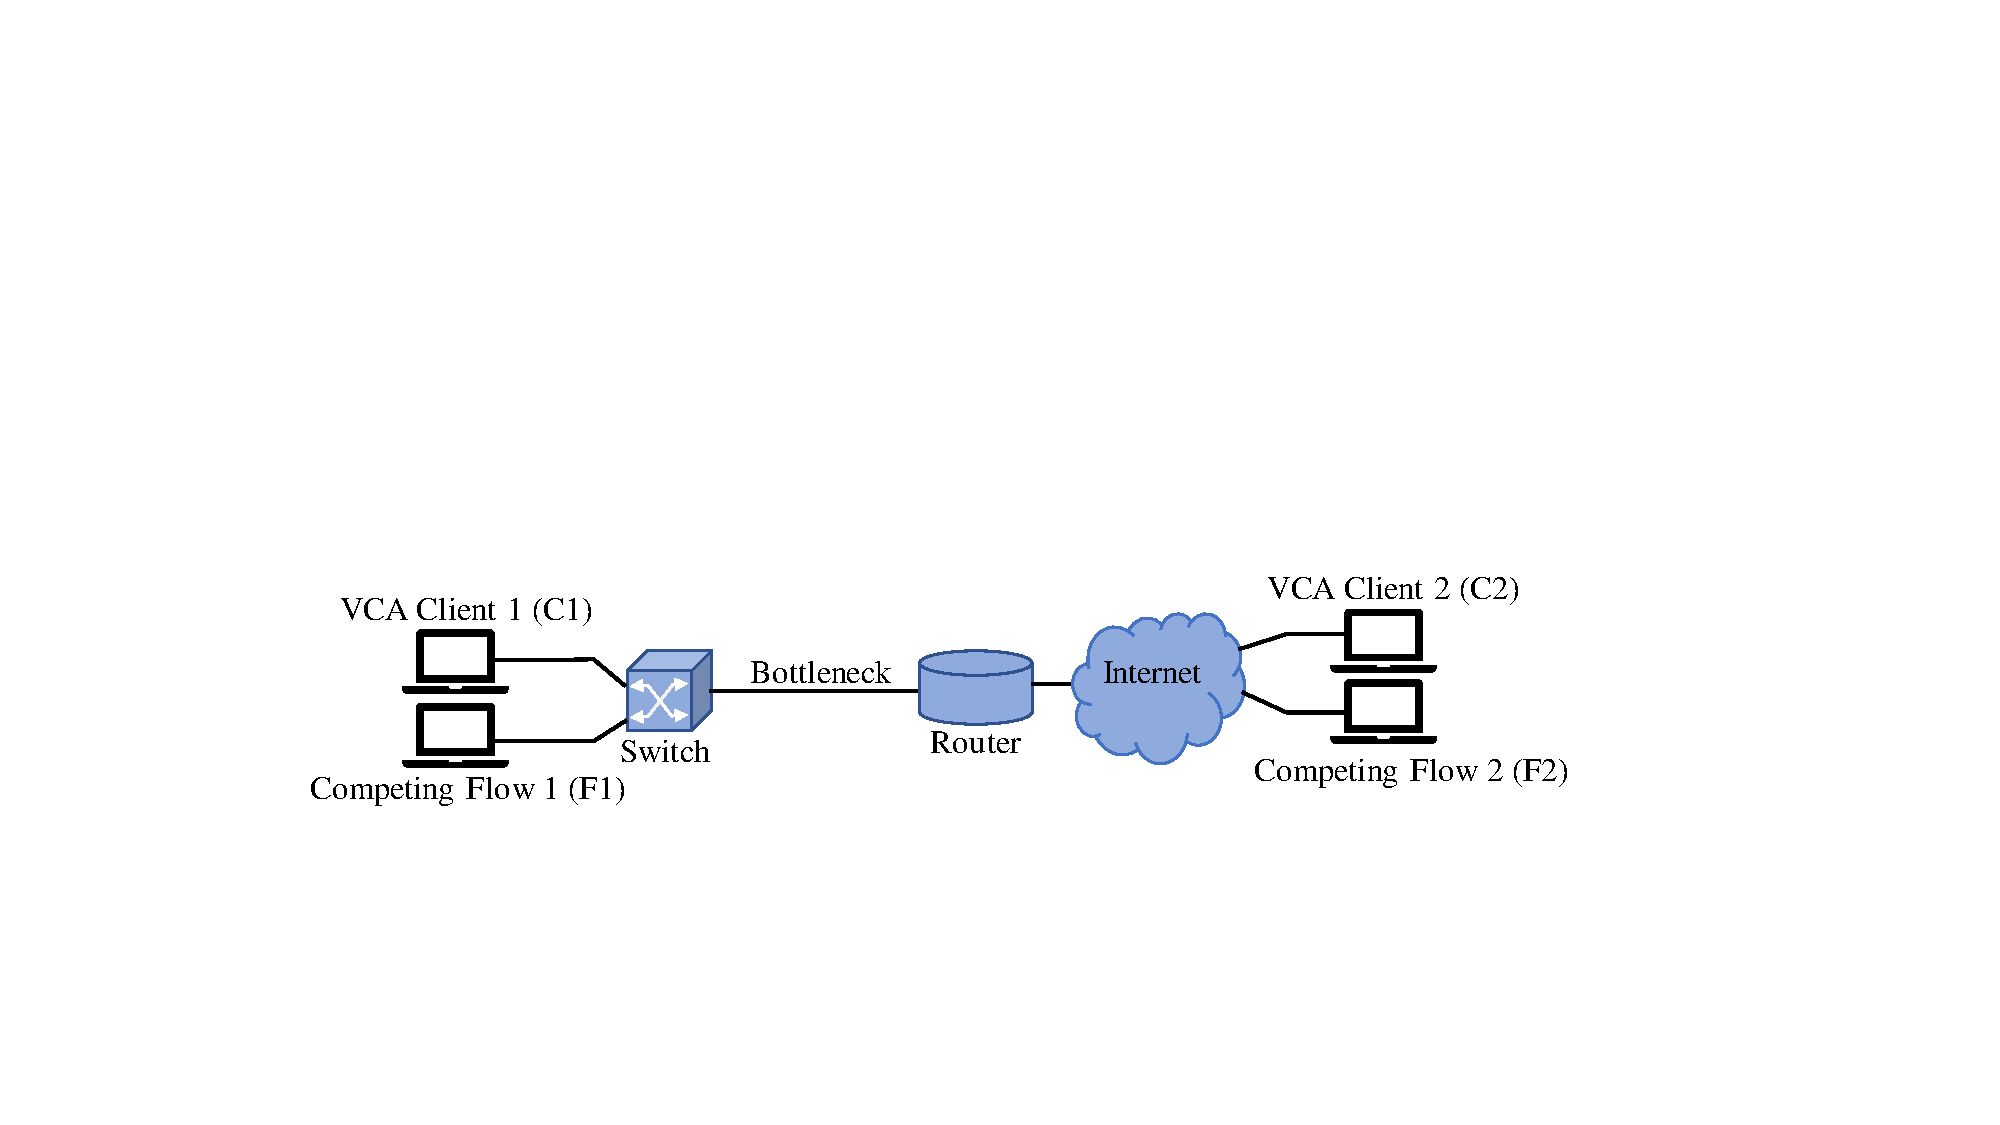
\includegraphics[width=0.5\textwidth,keepaspectratio]{../figures/methodology/competition-setup.pdf}
    \caption{Setup for competition experiments
    }
    \label{fig:loss_latency}
\end{figure}
 
\end{center}

The experiment is built within the framework already described.
The distinguishing feature of this measurement is that the 
  constrained link is between a switch and an OpenWRT Router 
    (which constrains the link).
The router has a gigabit link to the Internet.
The competing flows are initiated from two matched consumer laptops,
  connected to the switch over unconstrained, gigabit links.
We consider three forms of competitive flows:
  a standard TCP flow through iperf3 with cubic congestion control,
  other video conferencing applications, and 
  common video streaming services.
The ``counter-parties" for these flows are, respectively,
  a dedicated server on the university network,
  consumer laptops, and industry servers.
In contrast to previous experiments, 
  we focus on the native versions of Zoom and Teams clients.
\jamie{Awkward: Meet is native in Chrome.}

Each single experiment lasts for 4 minutes.
The ``nominal flow" is established first, and
  and the competing flow follow 30 seconds later.
The competing flow lasts for 2.5 minutes.
The experiment concludes with 1 minute
  with the nominal flow alone.
This setup is illustrated in Figure~\ref{fig:ts_zoom_netflix},
  with the time series for a six experiments between Zoom and Netflix.
Each configuration of nominal and competing flows and link constraint
  is repeated five times.
The capacity constraints are to 0.5, 1, 2, 3, 4, and 5 Mbps.
Bitrates are measured from packet captures.
  
\begin{figure}[]
    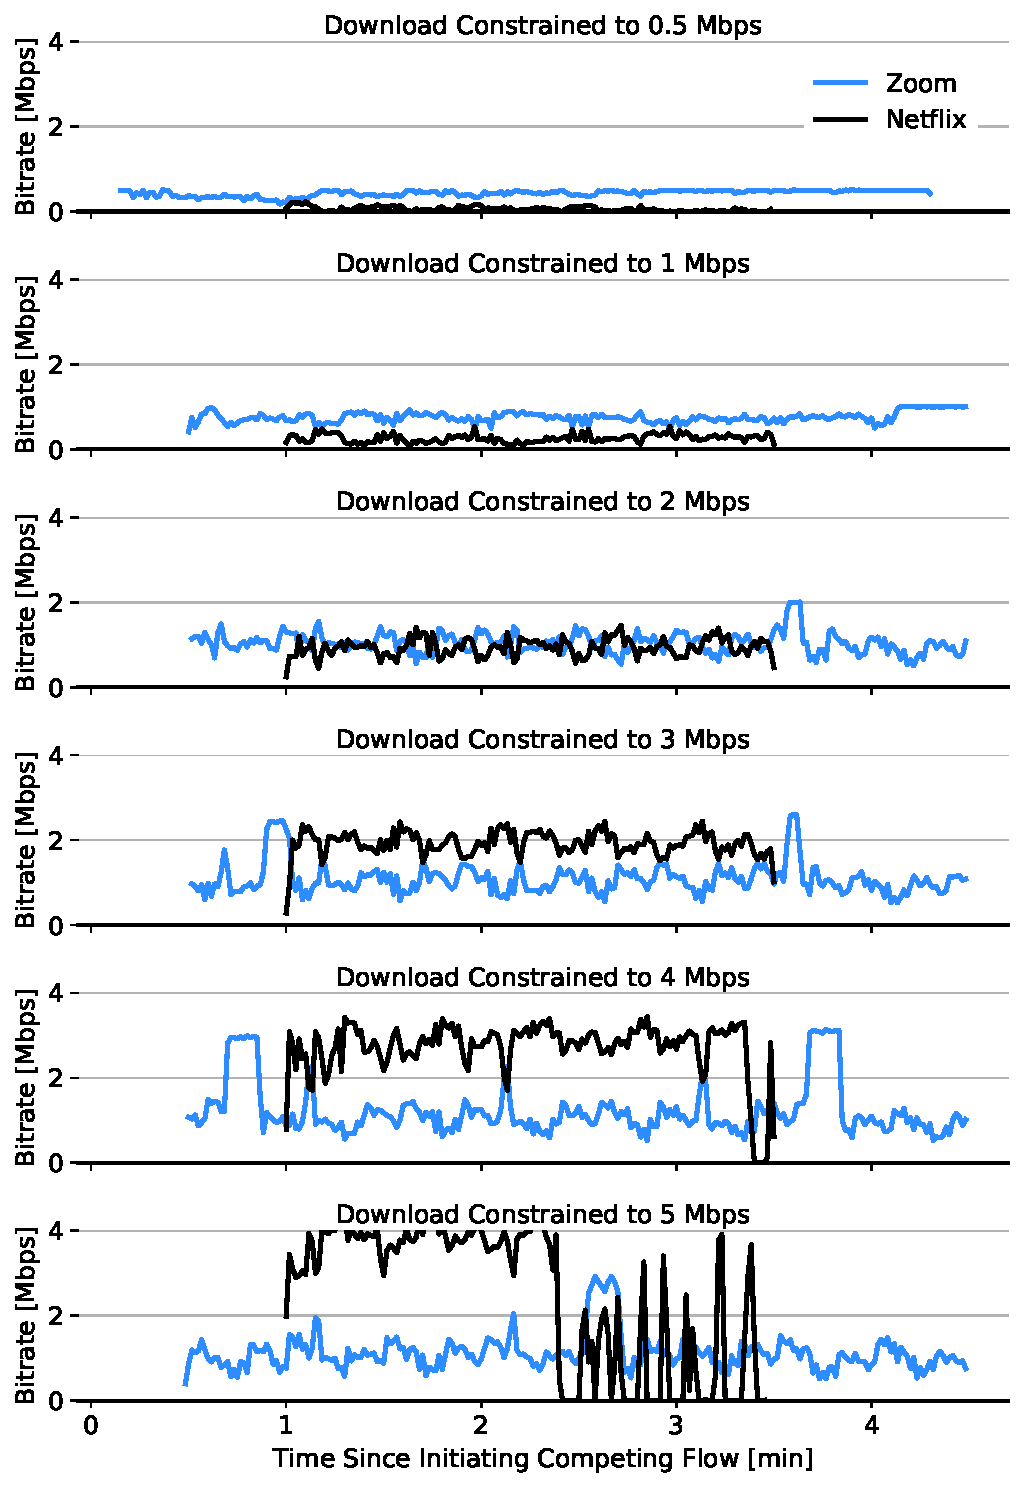
\includegraphics[width=\linewidth]{comp/zoom_netflix_dl_time_series.pdf}
    \caption{Time series of bitrate for Zoom in competition with a Netflix flow, at different link capacity. \jamie{timing offset bug}}
	\label{fig:ts_zoom_netflix}
\end{figure}

\begin{figure}[]
    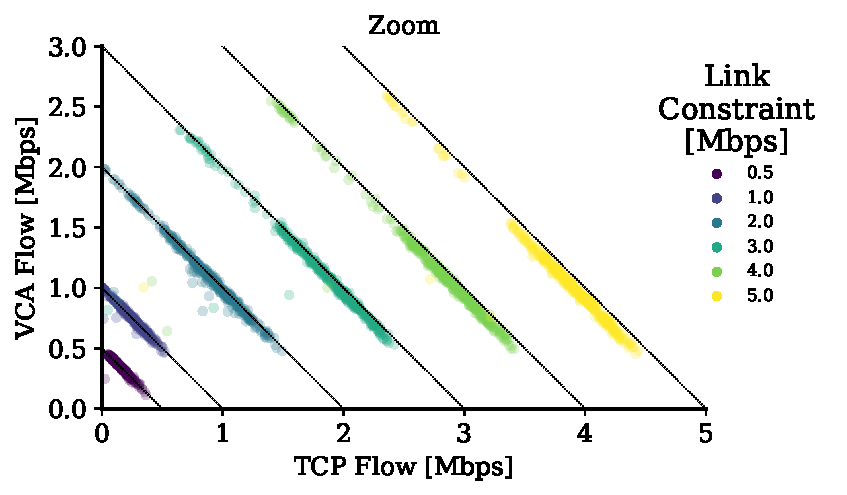
\includegraphics[width=\linewidth]{comp/zoom_iperf_scatter.pdf}
    \caption{Competition between Zoom and an iperf3 TCP flow. \jamie{kind of pretty, but not obviously useful}}
	\label{fig:comp_zoom_iperf}
\end{figure}

\begin{figure}[]
    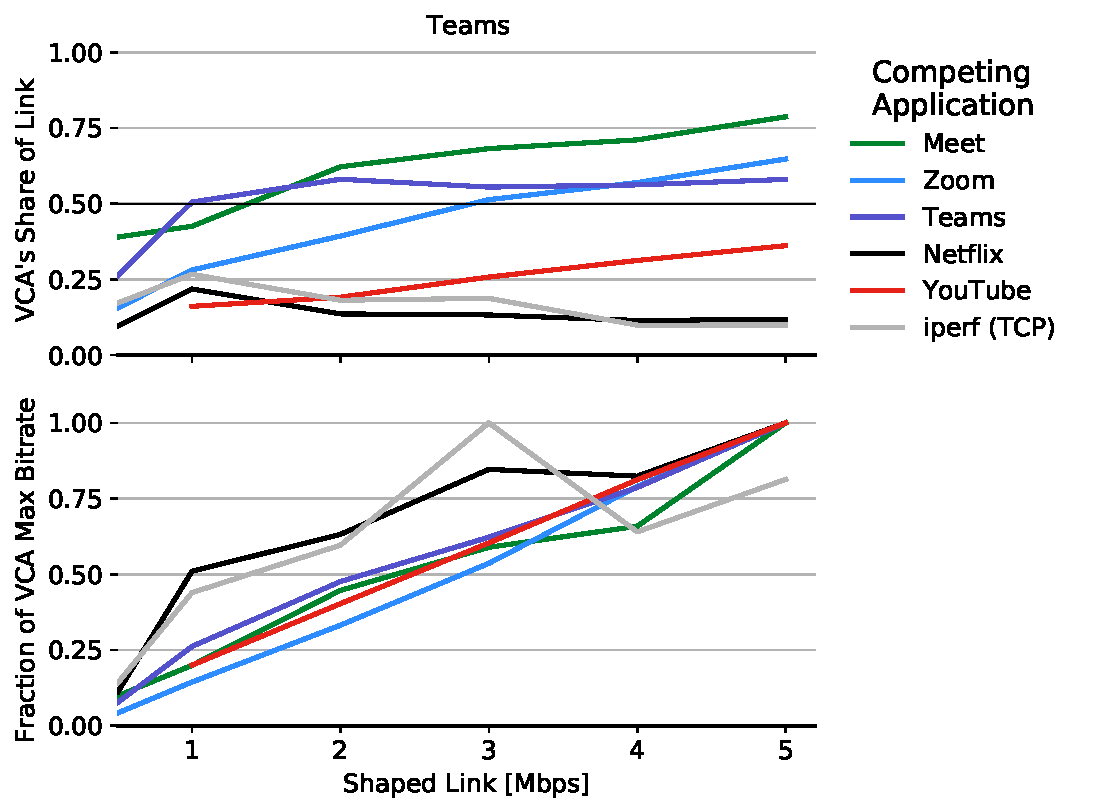
\includegraphics[width=\linewidth]{comp/teams_competition.pdf}
    \caption{Link share and share of nominal bitrate for Teams, in competition with other flows, as a function of downlink bitrate cap. \jamie{Combine this and following figures into one full-width / 6-panel figure.  Increase font sizes, etc.}}
	\label{fig:teams_comp_bitrates}
\end{figure}

\begin{figure}[]
    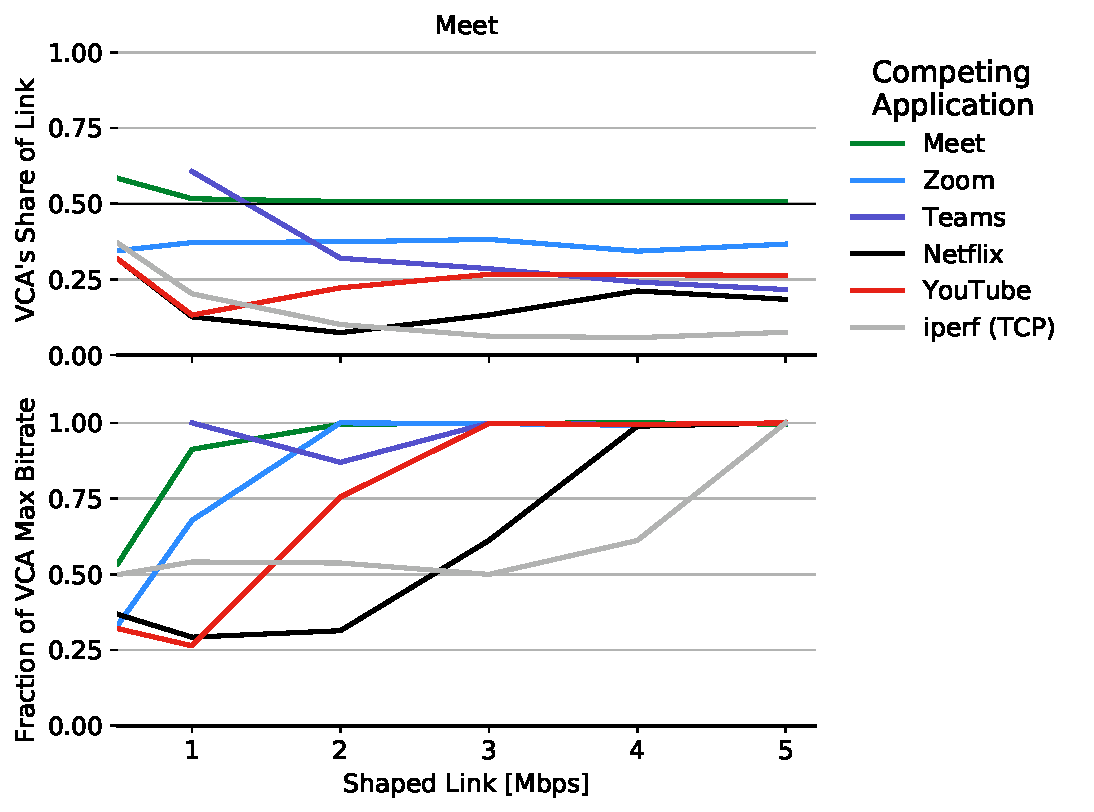
\includegraphics[width=\linewidth]{comp/meet_competition.pdf}
    \caption{Link share and share of nominal bitrate for Meet, in competition with other flows, as a function of downlink bitrate cap.}
	\label{fig:meet_comp_bitrates}
\end{figure}

\begin{figure}[]
    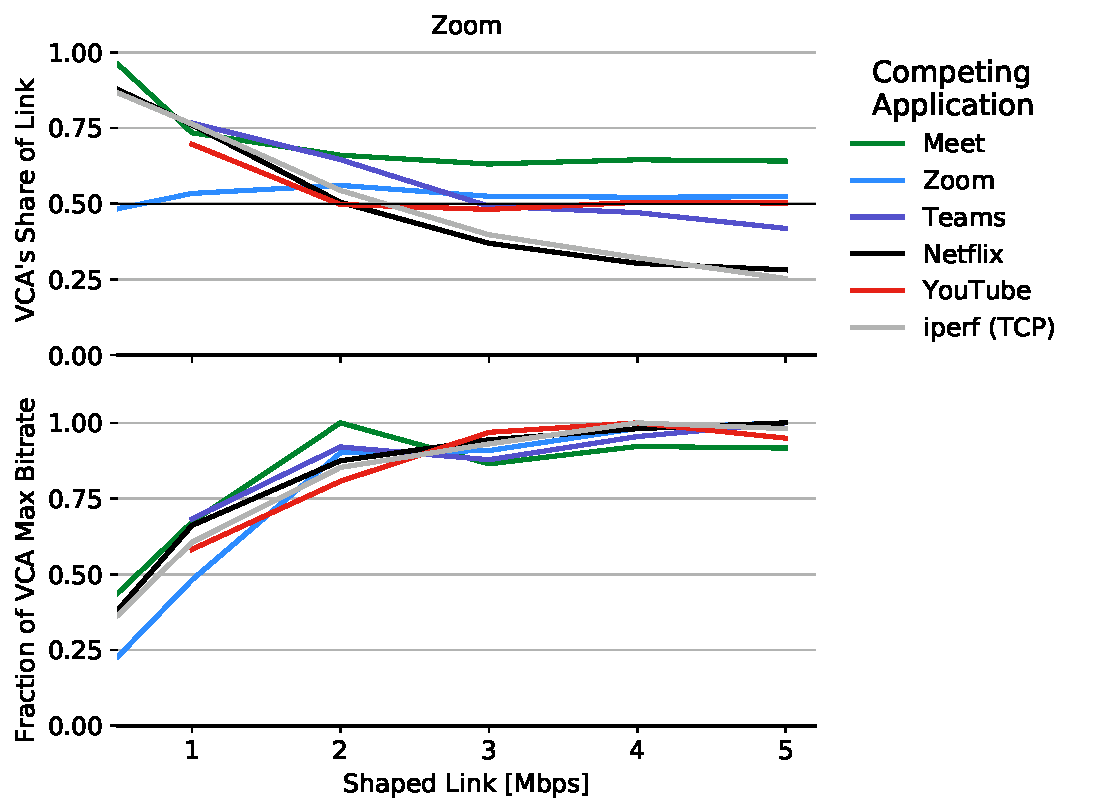
\includegraphics[width=\linewidth]{comp/zoom_competition.pdf}
    \caption{Link share and share of nominal bitrate for Zoom, in competition with other flows, as a function of downlink bitrate cap.}
	\label{fig:zoom_comp_bitrates}
\end{figure}

\begin{figure}[]
    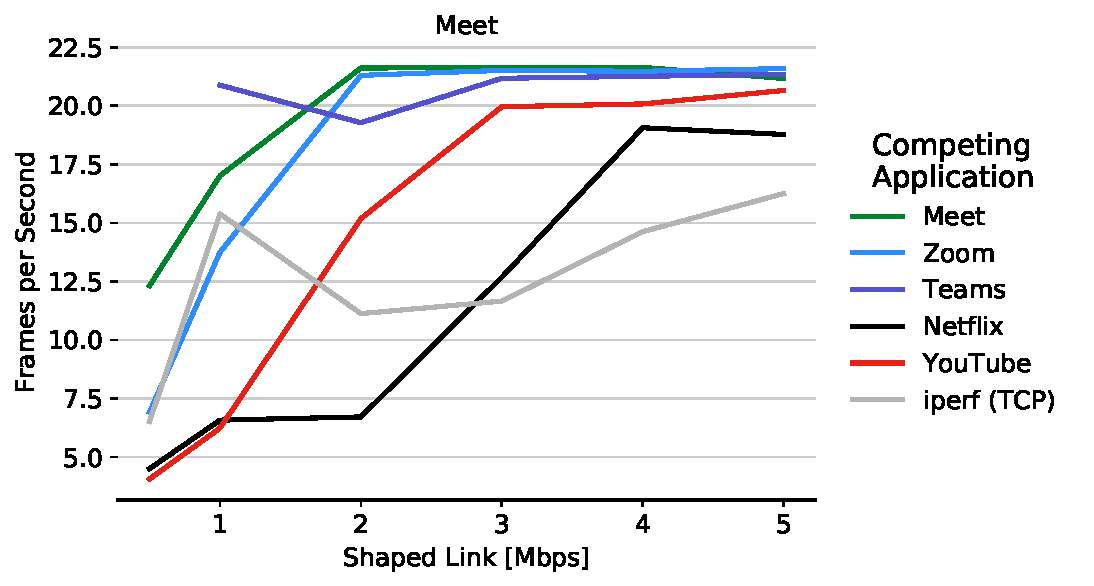
\includegraphics[width=\linewidth]{comp/meet_performance.pdf}
    \caption{Meet frames per second, in competition with other flows and as a function of link capacity.}
	\label{fig:meet_comp_performance}
\end{figure}



From these flows we construct two variables
  to reflect fairness and performance.
Fairness is represented 
  as the nominal flow's share of the constrained link.
Performance is the flow's share of its bitrate 
 as measured on a fully unconstrained call (see Table~\ref{}).
\jamie{The fully-unconstrained values are important benchmarks that we should measure carefully.  I know Tarun quoted these.  But we should establish these and put them in a table early on.}
Figures~\ref{fig:teams_comp_bitrates}-\ref{fig:zoom_comp_bitrates}
  display results for Teams, Meet, and Zoom respectively.

Each application in ``competition" with itself, uses half the link.
Competition is in evidence primarily at the low end of the domain,
  with the most severe constraints.
With weaker constraints, most applications reach their nominal bitrates
  and the ratios in the upper panels simply show the ratio of their bandwidth demands.
For example, 
  the low VCA shares with respect to iperf at weak constraint
  simply illustrates the "inexhaustible" demand of a TCP flow,
  whereas link share's of Zoom vs Meet or Meet vs Zoom 
  at link capacity of 5 Mbps (0.4 or 0.6) simply 
  reflect the nominal bandwidths.

\jamie{ambiguity: NetFlix or YouTube buffering, vs slow-start from teams}
  
At the low end, Zoom competes
  aggressively and effectively with all other flows:
  it consumes nearly the entire link against Meet (\textcolor{red}{95\%}), 
  and \textcolor{red}{80\%} of the link against Teams.
Both Teams and Meet fare worse on constrained links.
  
The lower panels of the figures show
  the link bandwidth required for the VCAs' consumption
  to converge to their nominal levels.
Again, Zoom is quick out of the gate, and 
  achieves over \textcolor{red}{90\%} of nominal link bitrate,
  for constraints weaker than 2 Mbps.
On the other hand, Teams does not achieve full bitrate
  until \jamie{we gotta run higher..}
Depending on the flow, Meet achieves full 
  performance when the shared link has capacity greater than 3 Mbps, 
  except for the (unlimited) TCP flow.
  
\jamie{Zoom competing with meet nominal is flat, whereas the inverse is not.  These aren't exactly the same -- there's an ``incumbency" advantage -- but worth noting.}

\jamie{Add notes on performance, e.g., through Meet, though I think that the preceding is most of the story.}


% \begin{figure}[]
%     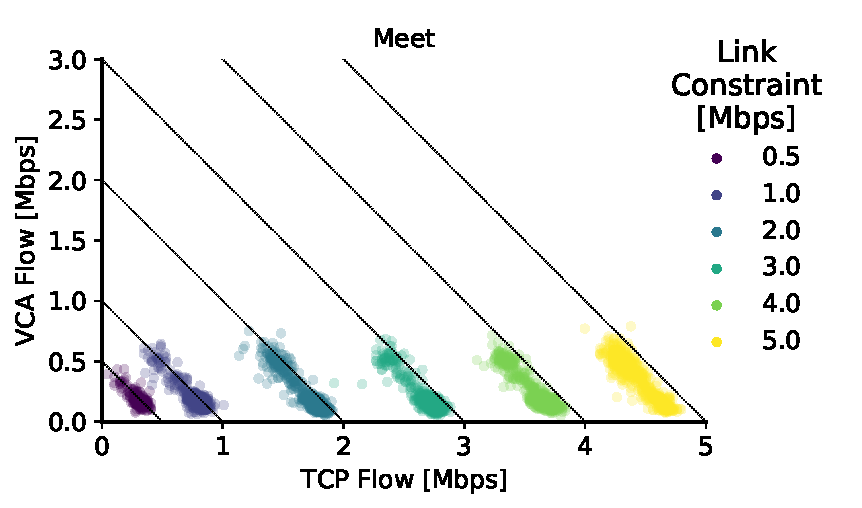
\includegraphics[width=\linewidth]{comp/meet_iperf_scatter.pdf}
%     \caption{Competition between Meet and an iperf3 TCP flow.}
% 	\label{fig:comp_meet_iperf}
% \end{figure}

% \begin{figure}[]
%     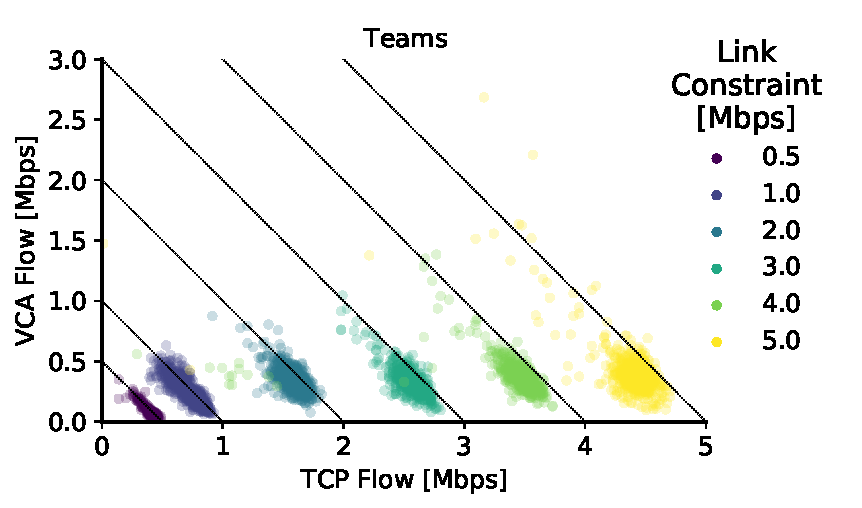
\includegraphics[width=\linewidth]{comp/teams_iperf_scatter.pdf}
%     \caption{Competition between Teams and an iperf3 TCP flow.}
% 	\label{fig:comp_teams_iperf}
% \end{figure}

